% !TEX root = ../rawlik-phd-thesis.tex
\chapter{Axion analysis}
\label{ch:axion-analysis}

Now that the foundation of the analysis has been explained we proceed to present how were they applied to the data. The data have been taken at PSI in the years 2015-17 during nEDM runs (as in no dedicated runs have been done.)

Explain why short and long time-base analyses. Mention the axion wind analysis already.

In this analysis two couplings were considered. The first is scalar and looks like an oscillating nEDM. The second is vector and acts like an oscillating magnetic field.

The analysis has been divided in two based also on an another criterion. The long time--base and short time--base. The first used the data set of the nEDM experiment performed in ILL by the Sussex--RAL--ILL collaboration and covers oscillation periods up to days. The short time--base analysis used the PSI data set. The latter is the subject of this work, the former is part of the doctoral thesis of Nicholas Ayres \mnote{Cite Nick's PhD here}. We have closely collaborated.



\section{How a signal would look like}
It is instructive to first understand well how would an axion signal come up in the data.

The main purpose of the experiment is to measure the static neutron electric dipole moment. This would appear as a shift in $R$\mnote{Needs to be clear that the reader is familiar with $R$ here.} dependent on direction of the electric field relative to the magnetic one. In zero electric there would be no shift, while the parallel and anti--parallel configurations of the magnetic and electric fields would shift $R$ in opposite directions. Due to the data blinding
\footnote{In order to reduce bias the data were modified upon being taken in a way, that a secret nEDM was injected into them. This additional offset is only revealed as the very last step, once the measurement and analysis have been completed. The data were still blinded at the time of writing.}
we expect a pronounce shift corresponding to an nEDM of \SI{e-25}{\elementarycharge\centi\meter}.

Should the neutron electric dipole moment oscillate, $R$ would oscillate as well, even if the electric field is kept constant. A reversal of the electric field polarity would reverse the phase of the oscillations. At zero electric field no oscillations would be visible. In Fig.\,\ref{fig:axions_data_taking_one_run} we depict an $R$ time--series with the combined effect of a large nEDM oscillation and the blinding offset.

\begin{figure}[bth]
  \myfloatalign
  \subfloat
  [An oscillating neutron electric dipole moment signal in the nEDM @ PSI apparatus. The colours indicate different electric field states: parallel to the magnetic field, antiparallel to it and zero]
  {\label{fig:axions_data_taking_one_run}
  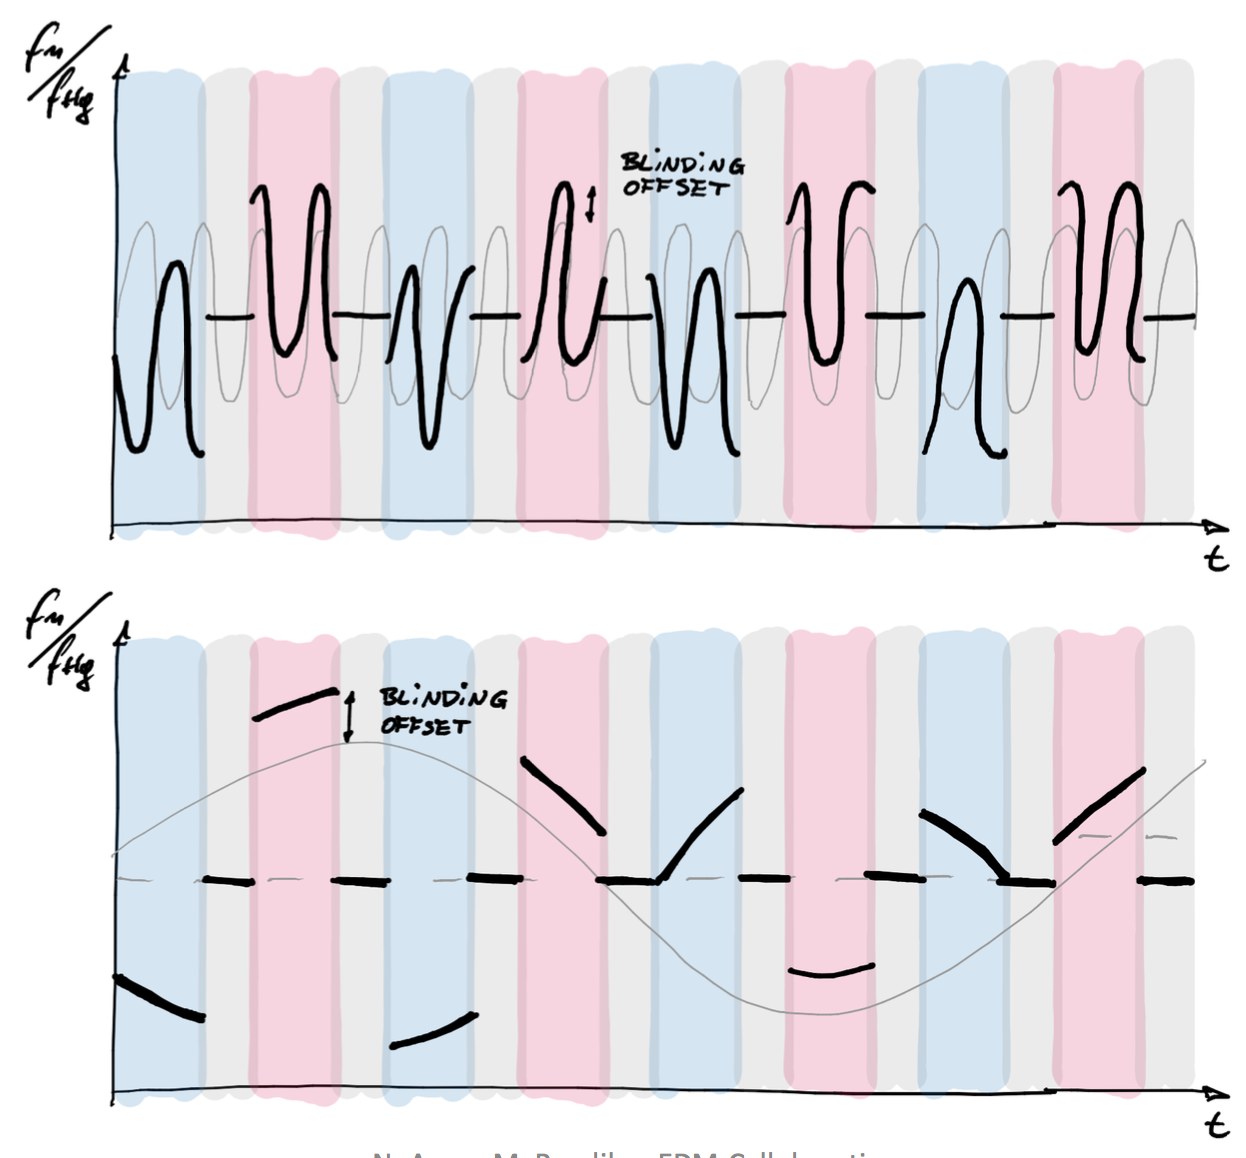
\includegraphics[width=.34\linewidth]{gfx/axions/cycle-level_blinding_offset.png}}
  \quad
  \subfloat
  [An oscillating neutron electric dipole moment signal in the nEDM @ PSI apparatus across many runs. The colours indicate different electric field states: parallel to the magnetic field, antiparallel to it and zero. Different runs have different magnetic field gradients, which causes each run to have a different shift in $R = f_n / f_{Hg}$.]
  {\label{fig:axions_data_taking_runs}
  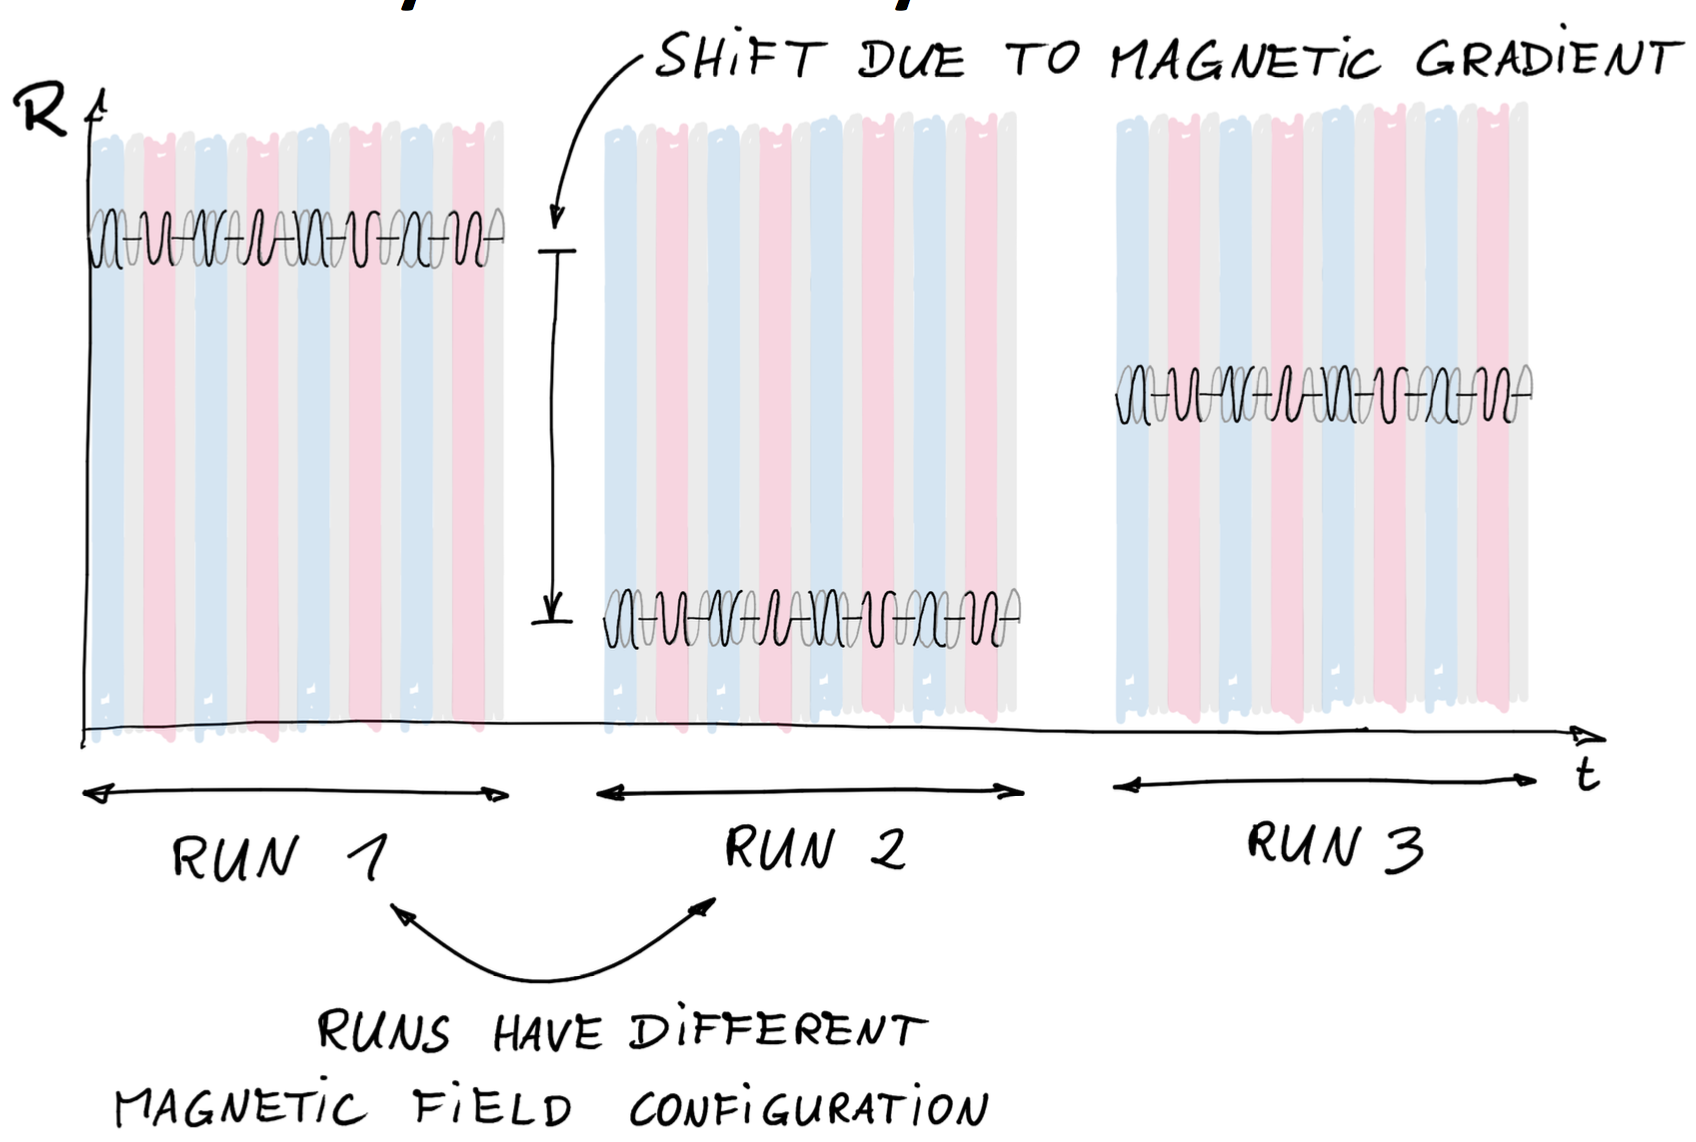
\includegraphics[width=.56\linewidth]{gfx/axions/cycle-level_gradient_jump.png}}
  \caption{The data taking scheme in the nEDM experiment at PSI.}
\end{figure}

A part of the measurement procedure is to deliberately work in a magnetic field gradient, as explained\ldots \mnote{Need to explain in somewhere, best at the beginning.} The vertical magnetic filed gradient changes substantially when a new run is started. \mnote{Give the reasons why it changes: we apply a new one, which follows from the measurement procedure} Thereby $R$ is shifted by a big value, changing the DC level of the oscillating nEDM signal, which is illustrated in Fig.\,\ref{fig:axions_data_taking_runs}. Moreover, even during a single run the gradient drifts, as clearly visible in Fig.\,\ref{fig:axions_gradient_drift_correction}. \mnote{Write here, that we can do a good relative gradient drift correction, but not an absolute one.}

\begin{figure}[bth]
  %FIXME directly copied from Elise's presentation on the 2015 PSI collaboration meeting
  \myfloatalign
  \subfloat
  [Another time series of $R$ in the nEDM experiment. The colours depict electric field states, black being no electric field. A drift is clearly visible.]
  {\label{fig:axions_gradient_drift_not_corrected}
  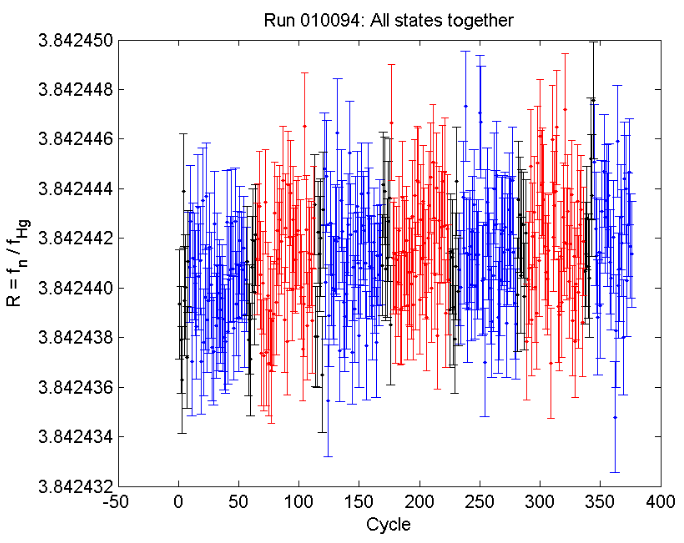
\includegraphics[width=.45\linewidth]{gfx/axions/gradient_drift_elise}}
  \quad
  \subfloat
  [The data as on Fig.\,\ref{fig:axions_gradient_drift_not_corrected} corrected for gradient fluctuations.]
  {\label{fig:axions_gradient_drift_corrected}
  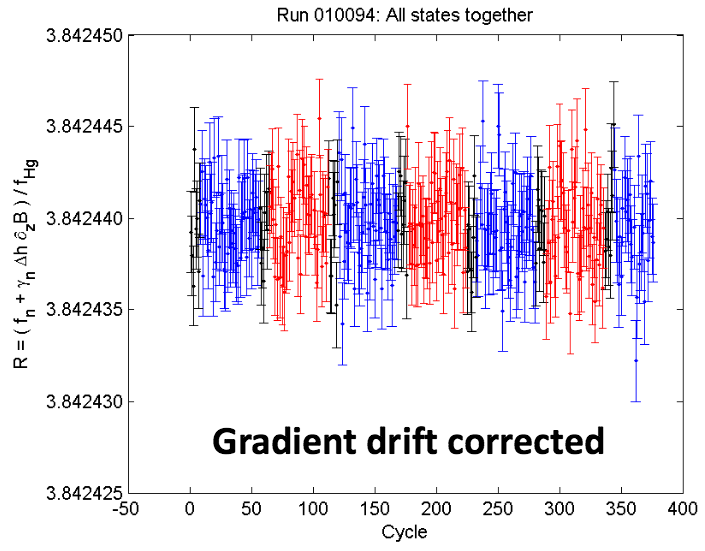
\includegraphics[width=.45\linewidth]{gfx/axions/gradient_drift_elise_corrected}}
  \caption{Correcting the $R$ time series for fluctuations of the vertical magnetic field gradient.}
  \label{fig:axions_gradient_drift_correction}
\end{figure}

The nEDM team spares no effort to measure the gradient. Nevertheless, the achieved precision (\SI[per-mode=symbol]{\approx 1}{\pico\tesla\per\centi\meter}) is only comparable to the one of $f_n$ (in the order of \SI{1}{\pico\tesla}). The exact way how the gradient should determined is highly non--trivial and there is ongoing research in this respect. \mnote{Mention here the exact way the gradient drift correction is done. And cite Elise's thesis.} Actually, even the height difference between the neturons and $^{199}$Hg centres of mass (a few milimeters) is still discussed. \mnote{Know how exactly was $\Delta h$ determined in the end. Also, mention the definition of a sequence here (as in the paper).} % Assuming a constant gradient during a \emph{run} one can determine it much more precise. This assumption, however, is known not to be exactly true.

One should note, that any, including an oscillating one, nEDM effect affects only the position of the neutrons' resonance. The shape of the resonance curve is unaffected. Therefore, the method to extract neutron Larmor frequency $f_n$, and thereby $R$, for each \emph{cycle} is valid also in case of an oscillating nEDM.

It may be tempting to think about demodulating the $R$ time--series into what would be expected to be an oscillation. This would require subtracting the DC offset for each electric field configuration, in each run separately, then flipping the signal around the DC level for one configuration. \mnote{The offsets are measured with Cs, mention that.} The disadvantage is that uncertainty in such a demodulation would become a systematic effect and would need to be tightly controlled.

A different approach, one that that was taken, is to split the $R$ time--series into three sets: without the electric field (a control data set, no signal expected), with the electric and magnetic field parallel, and with anti-parallel (the signal is expected to come up with an opposite phase in the two). Then in the LSSA fit instead of one DC offset, allow a different one for each run:
\begin{equation}
  \label{eq:axions_LSSA}
  A\sin(2 \pi f t) + B\cos(2 \pi f t) + \sum_i C_i\,\Pi_i(t) \,
\end{equation}
where $C_i$ is the free offset in the $i$th sequence and $\Pi_i(t)$ is a gate function equal to one in the $i$th sequence and zero elsewhere.
\mnote{The sensitivity deserves a separate paragraph somewhere later in the text.}






\section{Systematic Studies for the Cycle--Level Analysis}
While the run--level analysis can benefit from all of the systematic studies done for the constant nEDM measurement, this is not the case for the lower level cycle--level analysis. An important decision has to be taken on how to treat the systematic effects. There are three options:
% \begin{enumerate}
%   \item Perform a detailed study of time--dependent systematic effect.
%   \item Determine \emph{delicate} frequencies and cut them out.
%   \item Assume there are no systematic effects.
% \end{enumerate}

\paragraph{Perform a detail study of time--dependent systematic effect.}
Here we would assume that any excess in power, in any dataset ($E \uparrow \uparrow B$, $E \uparrow \downarrow B$ and $E=0$) is a signature of some kind of a signal. All effects that can potentially result in that should be identified before the analysis is performed and corrected for. This would require a long and careful systematic study, a task much bigger then this analysis itself. Moreover, the full--fledged systematic studies for the constant nEDM analysis of the PSI data are still ongoing. Even though we acknowledge that this would be \emph{the} proper way to go, we consider it to be unrealistic and unnecessary for this analysis.

\paragraph{Determine \emph{delicate} frequencies and cut them out.}
Looking at periodograms of raw data one sees that there are several typical frequencies where peaks appear. Typically at inverse specific time constants at which the experiment operates: cycle separation, day, week, , HV--reversal, B0--reversal. We may decide that all systematic effects are constrained to these frequencies and do not perform the analysis there at all.

\paragraph{Assume there are no systematic effects.}
An axion would produce a very specific signal, in particular:
\begin{enumerate}
  \item There would be no signal in the $E=0$ dataset.
  \item The signal would appear in both $E~\uparrow~\uparrow~B$ and $E~\uparrow~\downarrow~B$ datasets, with equal amplitude.
  \item The signals in $E \uparrow \uparrow B$ and $E \uparrow \downarrow B$ would be shifted in phase by 180~degrees.
  \item The signals would have to have a high coherence of $\delta f / f = 10^{-6}$.
\end{enumerate}
In case we see an excess in power, we would only call it a candidate for an axion--signal if the three above conditions are met. Otherwise we attribute it to a, potentially unknown, systematic effect. We do realise the danger of making the systematic search dependent of the act of finding a signal. This automatically opens a line of attack on this analysis: we would not make a discovery, because a systematic effect has canceled the real signal out. We would not have seen a signal and therefore not looked for systematic effects. This is certainly valid. Nevertheless, we argue that the extremely low probability of this event, due to the high coherence of the axion field, makes it negligible. In order to cancel the axion signal, a systematic effect would not only need to be as coherent as the axion field, but additionally fine--tuned over at least 5 orders of magnitude magnitude of tested frequencies. With the coherence of $\delta f / f = 10^{-6}$ this is a tuning of $10^{-30}$. It would also need to be fine--tuned in amplitude over $\sim 20$ orders of magnitude, which gives a rough estimate of the cancellation probability: $10^{-50}$. As we are presenting limits with 95\% C.L., we feel this approach is justified.

Out of the three, we opt for the third option, but leave the subject open to discussion for the collaboration.








\section{The PSI 2015-16 data set}
The PSI data set is taken 2015-07-03, 14:21:30 to 2016-12-18, 19:51:23. It has been a regular nEDM run. Per cycle one $R = f_\mathrm{n} / f_\mathrm{Hg}$ estimate is obtained. The complete data set used in the analysis is shown in Fig.\,\ref{fig:PSI_dataset_time_domain}.

\mnote{Idea: present a scheme of the timing structure of the nEDM data taking, where a cycle, sequence are defined, and HV and B field reversals are shown.}
The time structure ias follows: The atomic measurement is called a cycle, which gives an estimate of the average precession frequency of the neutrons $f_\mathrm{n}$ and mercury $f_\mathrm{Hg}$. Their ratio $R = f_\mathrm{n} / f_\mathrm{Hg}$ is show in Fig.\,\ref{fig:PSI_dataset_time_domain}. An automatic system executes one cycle after another (triggered on a signal from the UCN source). A series of automatically executed cycles is called a \emph{run}. The $R$ time series of a typical run, 1-3 days long, is shown in the lower-right corner. During a run the electric field automatically changes polarity every \ldots \mnote{Find out how many cycles for one HV cycle} cycles. In between \ldots cycles with no electric field are measured. These have no sensitivity to the electric dipole moment, but provide a control data set.

A run is taken always in one magnetic field configuration. No change of the trim coil currents.\mnote{Explain the R-curve and crossing-lines analysis already in the beginning, so that it is clear that we measure in different magnetic field configurations. You do not need to know the timing structure of your data to do that. Mention the $R$ equation there!} During the measurements the vertical magnetic field gradient $\partial B_z / \partial z$ is modulated from cycle-to-cycle (up to \SI{60}{\pico\tesla} in \SI{10}{\pico\tesla} steps) so that related systematic effects (which scale linearily with the magnitude of the gradient) with it can be extracted and corrected for (see some equation that has been introduced at the beginning. These large changes in the vertical gradient cause the different runs to be scattered in the plot.

During a single run the magnetic field is kept as stable as the team can manage. The drifts of the homogeneous part of the field are cancelled in $R$, but the gradients are not. So drifts of the gradient directly cause changes in $R$. These, however, can be corrected for using the Cs magnetometers. They are mounted on the top and bottom electrode and they can be used to correct for the in-run gradient drifts. They do not provide an accurate measure of the gradient. \mnote{Remember the reasoning why the cross-run gradient-drift correction can't be done: to large a change and the calibration issues}.

Sometimes for technical reasons there is a pause in the measurements. Then the collected data may still belong to one run One such sequence is shown in the lower-right inset in Fig.\,\ref{fig:PSI_dataset_time_domain}.

Typically... Sometimes stopped... Define a sequence



Really, really first, show some example runs. 

\begin{figure}
  \centering
  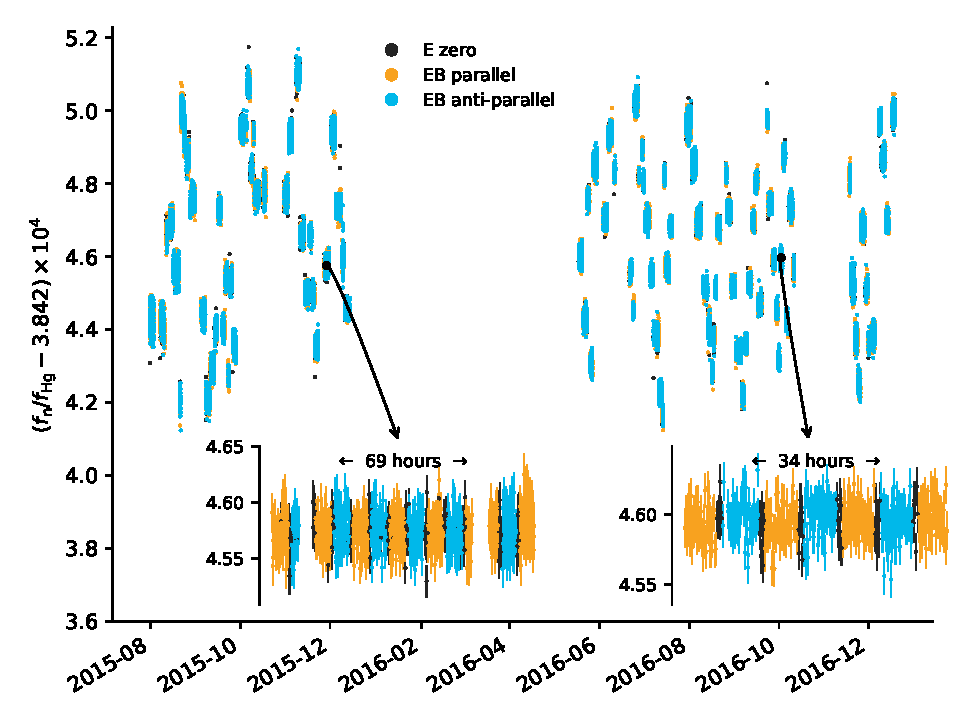
\includegraphics[width=0.9\linewidth]{gfx/axions/deltah4mm_time_domain_inset_no_yerr.pdf}
  \caption{The complete PSI data set used in the analysis. It spans from July 2015 to December 2016. Two sequences are enlarged. Due to high density of the measurements individual points cannot be resolved. The $R$ time series has been corrected for gradient drifts.}
  \label{fig:PSI_dataset_time_domain}
\end{figure}


\section{The analysis itself}

We start by presenting the results and then proceed to a more in-depth discussion.

\mnote{Definitely put in the plots for all three analyses (E0, EBp and EBap)! But only in the appendix!}

\mnote{This does not need to be explained really in detail! Most of the things were already explained earlier\ldots}

\mnote{The largest missing piece is the Cs gradient-drift correction. What should I do with it? The correction should be introduced by now!}

\begin{figure}
  \centering
  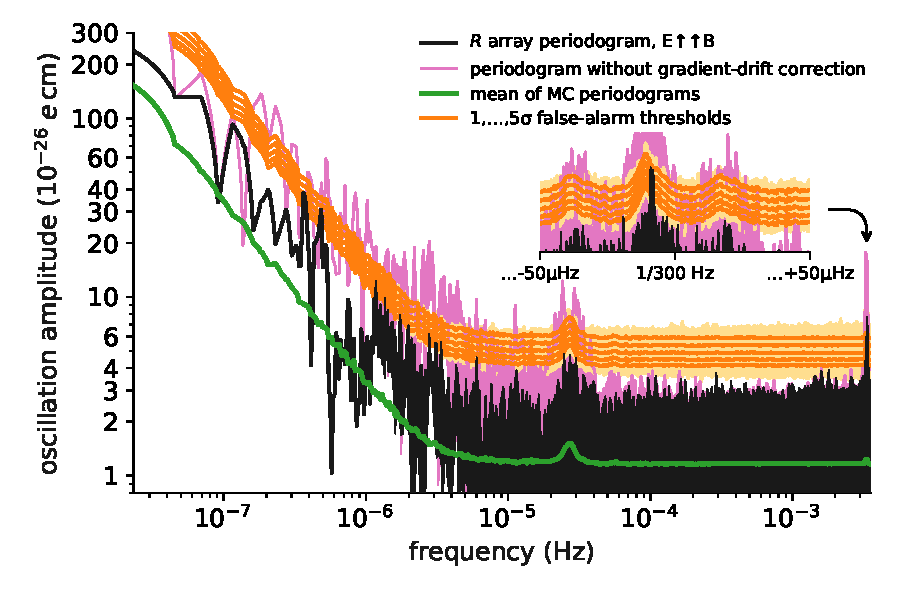
\includegraphics[width=0.9\linewidth]{gfx/axions/detection_psi_inset_gc.pdf}
  \caption{Periodogram of the $R$ time array of the PSI experiment data, sensitive to oscillations in the quantity $d_\mathrm{n} - \left( \mu_\mathrm{n} / \mu_\mathrm{Hg} \right) \, d_\mathrm{Hg}$, taken with the $\boldsymbol{E}$ and $\boldsymbol{B}$ fields parallel (black line).
  The mean of MC--generated periodograms, assuming no signal, is depicted in green. MC is used to calculate $1,2,…,5\,\sigma$ false--alarm thresholds, depicted in light orange.
  For clarity, we also plot the smoothed version in orange.
  There are two regions where a rise in the amplitude is expected, namely around \SI{28}{\micro\hertz} (inverse of 10 hours) and \SI{3.3}{\milli\hertz} (inverse of 300 seconds), due to the time structure of the data taking (see the main text for more details). The periodogram of non-gradient-drift-corrected data is shown in pink.}
  \label{fig:axions_PSI_detection}
\end{figure}

The periodogram of the subset of data with the electric and magnetic field parallel is presented in Fig.\,\ref{fig:axions_PSI_detection}.
There are two regions of expected rise in the oscillation amplitude due to the time structure of the data collection.
The one around $\unit[28]{\upmu Hz}$ (the inverse of 10 hours) corresponds to the period of the electric-field reversal.
The very narrow one around $\unit[3.3]{mHz}$ (the inverse of $\unit[300]{s}$) corresponds to the cycle repetition rate.
There are five
%\note{NA does anybody know what style guide says about when numbers should be written in words i.e. seven vs 7? I personally think small numbers without units should be words but this comes down to preference} ***I THINK LESS THAN TEN IT IS IN WORDS - MALCOLM ***
trial frequencies for which the $3\sigma$ false--alarm threshold is exceeded,
%\note{PMM: use words like 'surpassed', or 'exceeded' instead of penetrated}
two of which, including the largest excess with a $6\sigma$ significance, occur in a $\unit[100]{\upmu Hz}$ region around the inverse of \unit[300]{s}, while the other three are in the low-frequency region (inverse days) already excluded by the long time--base analysis.
% \note{FP: Can you maybe also explicitly state the positions of these three lines in Hz or inverse time?}
 The periodograms for the other two datasets (presented in \ref{ch:alp_appendix}) are very similar.
In the other sensitive set, there are three excesses of the $3\sigma$ threshold (the highest is $5\sigma$), all constrained to the same two regions. In the control dataset, only the $1\sigma$ threshold is exceeded.
%\note{MR: We may consider not discussing the false--alarm threshold penetrations, and just state in the next paragraph that we do not find a signal which meets our criteria.}
The periodogram of the $R$ time array without the gradient-drift correction is shown in pink in Fig.\,\ref{fig:PSI_detection} to visualize the frequencies where the correction has an effect.

\mnote{Here a brief discussion about the Cs-gradient-drift correction.}
It is interesting to observe, that the periodograms with and without the gradient drift correction diverge only for frequencies below \SI{6e-5}{\hertz}, the period of the high-voltage reversal (the disagreement around inverse \SI{300}{\second} is folded from the low frequencies). This is not a coincidence. The period of the high-voltage reversal has been deliberately chosen, so that\ldots\mnote{Was the period really chosen such?}

No signals fulfilling the detection criteria are found.

Having observed no significant signal, we could place limits on the coupling strength as the function of axion mass.
The result are presented in Fig.\,\ref{fig:axions_limits_coupling} and are labeled \emph{short time-base} (the next paragraph is devoted to the \emph{long time-base} limits).
The limits we evaluated using Monte Carlo techniques, as described \ldots.
The results are presented in the landscape of already existing limits: axions with a mass below \ldots have their Compton wavelength larger than the size of the smallest dwarf \emph{galaxies} and, therefore, could not be the sole constituent of dark matter; the influence of axions in the red-shaded area on the \emph{Big Bang nucleosynthesis} would result in an underproduction of\ldots .
\mnote{Need to research and explain all those.}

\begin{figure}
  \centering
  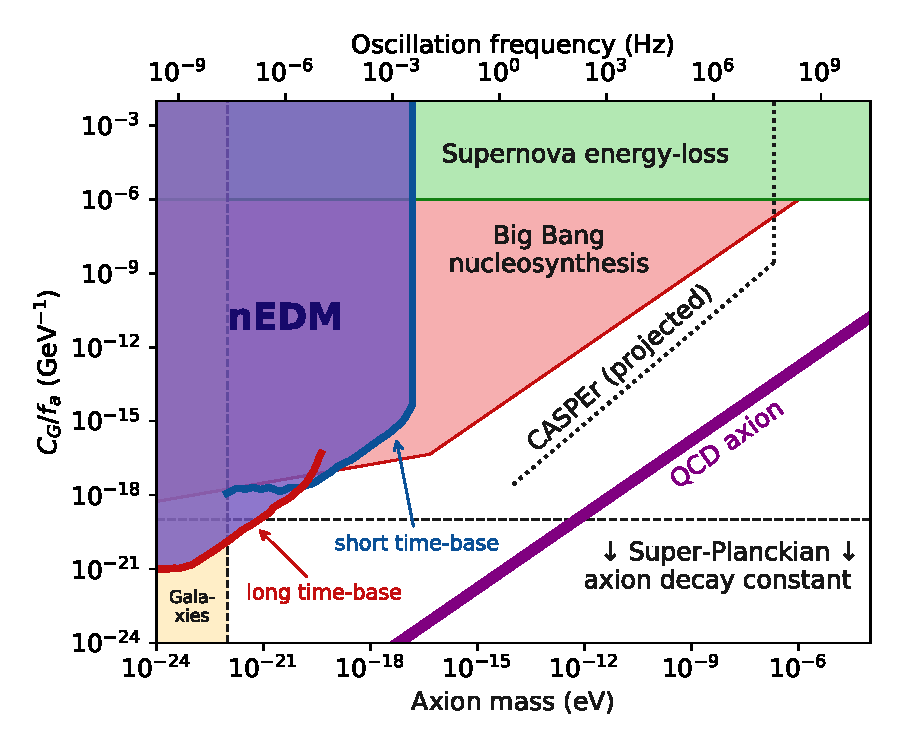
\includegraphics[width=0.9\linewidth]{gfx/axions/psi_ill_axion_limits_v7.pdf}
  \caption{Mention, that it shows\ldots}
  \label{fig:axions_limits_coupling}
\end{figure}

The Fig.\,\ref{fig:axions_limits_coupling} features the \emph{short time-base} limits, the ones described in this work, as well as \emph{long time-base} ones.
This work was performed with close collaboration with Nicholas Ayres of the University of Sussex. The Sussex group was part of the collaboration running the predecesor of the nEDM experiment at PSI --- the measurement performed in the Institute Laue-Langevin in Grenoble, France, in the years 1998--2002~\cite{Pendlebury2015}.
An analysis analogous to this work was performed on those data, with an important difference, which made it sensitive to lower frequencies (or lighter axions)~\cite{AyresThesis}.
Namely, the time series consisted of one point per run, in contrast to one per cycle in the short time-base analysis.
On one hand it limits the sensitivity to oscillation periods corresponding to one run (1--2 days).
On the other, the sensitivity to low frequencies is not deteriorated, as there is no need to use multiple free offsets in the LSSA fit (Eq.\,(\ref{eq:axions_LSSA})). In fact the free offset is assumed to be zero on the ground that the experiment delivered a zero-compatible result.
% in the process of calculating the per-run nEDM estimate the gradient fluctuations are averaged out, so there is 
\mnote{What about the gradient-related systematics (nEDM vs R' curve)? Was it corrected for? Wrote an email to Nick.}

Despite close collaboration the two analyses shared no common code. As a mean of cross-check, the two codes were compared on artifical datasets, more on that in the appendix.




\section{False-alarm thresholds}
\mnote{In this section we will dive in more deeply into statistics associated with the data.}

Remind: for each of the three data sets we have a periodogram, one value for the power estimate for each frequency. Then we have a collection of simulated periodograms, many power estimates for each frequency, generated assuming the null hypothesis --- only white noise in the data.

First how the local p-values were obtained. In Fig.\,\ref{fig:P_best_signal_candidate} the cumulative distribution function (CDF) \mnote{define CDF somewhere and then just continue to use it. Maybe even a table of abbreviations at the end?} of the power at one frequency (a special one, where the least probable peak is). CDF has this advantage over the PDF, that it does not require binning to be estimated. To estimate the CDF all the MC-generated power estimates are sorted into an array. Then the discrete CDF estimate is plotted by putting the power on the x-axis and the place in the sorted array, normalised to one, on the y-axis. Fig.\,\ref{fig:P_best_signal_candidate} actually shows $1 - \mathrm{CDF}$, so that the logarithmic y-scale can be leveraged to resolve the high-power tail. The plot also includes a extrapolating fit line and false--alarm thresholds, which we now proceed to explain.

\begin{figure}
  \centering
  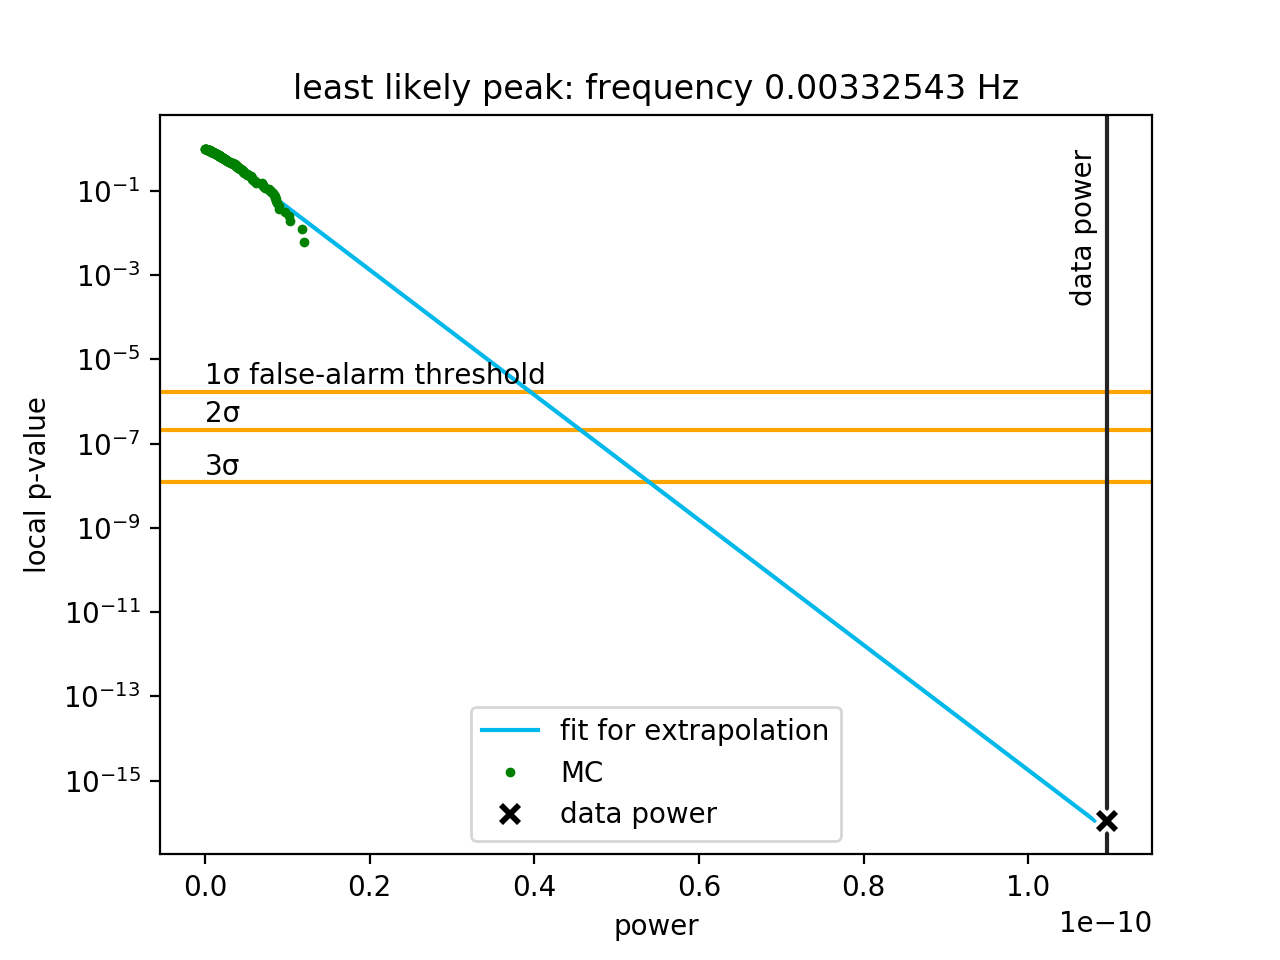
\includegraphics[width=0.9\linewidth]{gfx/axions/P_best_signal_candidate.png}
  \caption{1 - CDF for the parallel data set. This provides the power to local p-value transition, for each frequency separately. The extrapolation based on Eq.\ldots is shown.}
  \label{fig:P_best_signal_candidate}
\end{figure}

Once every MC-generated power estimate has a local p-value associated with it, we find for each generated periodogram the minimal local p-value and treat it as a statistic in itself. We estimate the CDF of the minimal local p-value. The result is plotted in Fig.\,\ref{fig:P_look-elsewhere}. The plot can be understood in the following way: it states how probable it is (y-axis) for a peak of a given local significance (x-axis) to occur anywhere in a periodogram. In other words, the y-axis corresponds to the \emph{global} p-value. The global p-value for an $n\,\sigma$ level is given by:
\begin{equation}
  \mathrm{erfc}\left( \frac{n}{\sqrt{2}} \right)\ ,
\end{equation}
where $\mathrm{erfc}$ is the complementary error function (intuitively understood as ,,one minus the integral of the gaussion distribution''). We mark the global p-values corresponding to $1,\ldots,5\sigma$ levels and via the CDF find the corresponding local p-value thresholds.

\begin{figure}
  \centering
  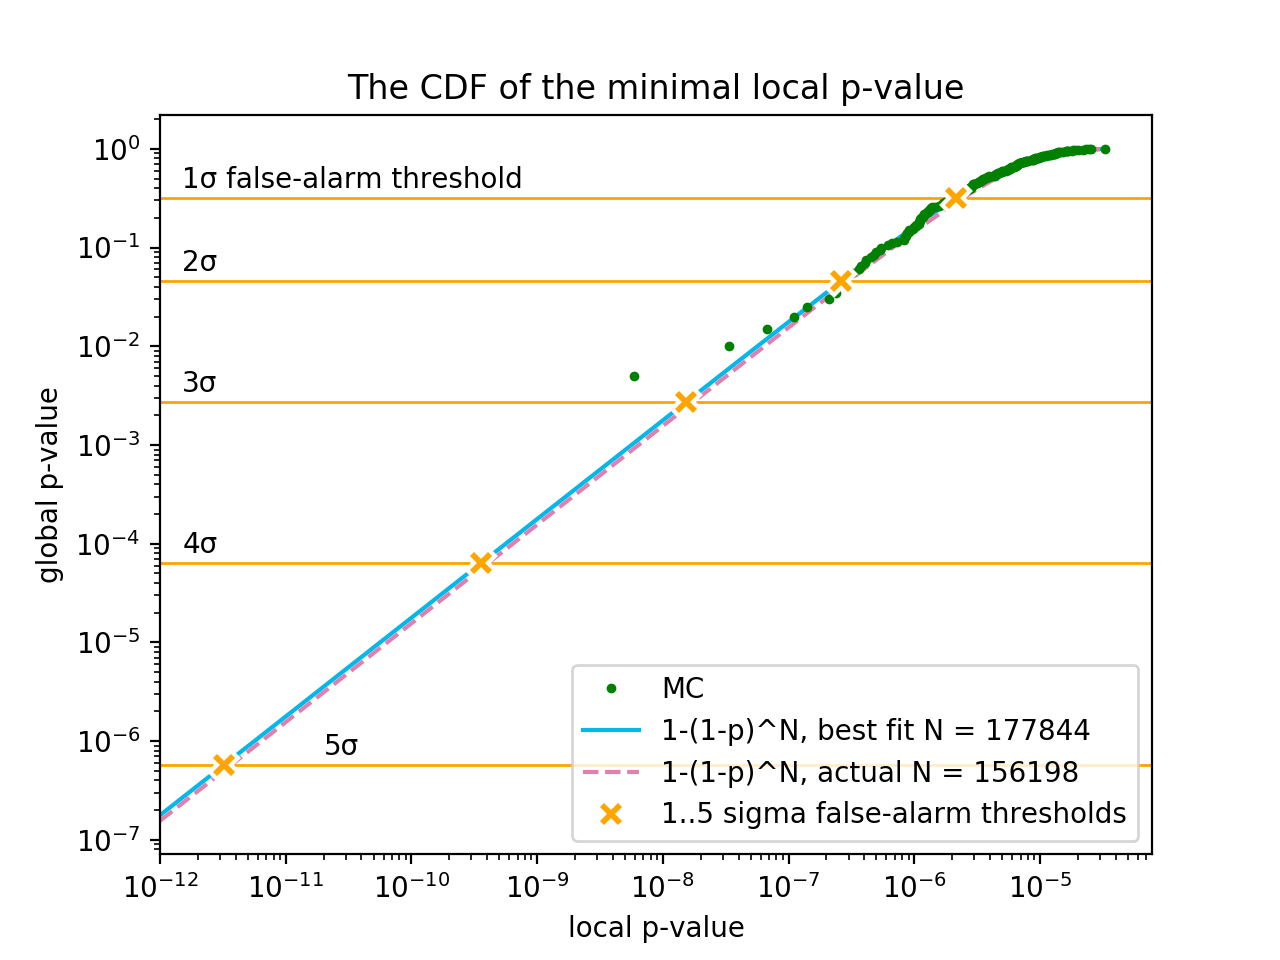
\includegraphics[width=0.9\linewidth]{gfx/axions/P_look-elsewhere.png}
  \caption{Accounting for the look-elsewhere effect for the parallel dataset. It provides the minimal local p-value -- global p-value transition. The fit with the model \dots gives the number of frequencies.}
  \label{fig:P_look-elsewhere}
\end{figure}

We see, that the discrete estimate from the MC simulation can only go down to the $2\sigma$ false-alarm threshold. To go lower would require many more MC samples. To observe a single $5\sigma$ event, roughly one-in-a-million, needs typically a million samples. To reduce the computational effort we exploit the fact, that we know the expected functional form of the CDF:
\begin{equation}
  F(p) = 1 - (1-p)^N\ ,
\end{equation}
\mnote{Ref. for the formula? PDF statistics? Scargle?}
where $N$ is the total number of frequencies. This corresponds to $N$ \emph{independent} statistical tests. We refrain from using for $N$ the actual number of frequencies, \num{156198}, because we cannot guarantee that the power estimates at different frequencies are independent\footnote{They are in a case of periodograms of evenly sampled series}. Instead, we fit $N$ to the observed CDF obtaining \num{177844}. CDFs corresponding to both values of $N$ are depicted in Fig.\,\ref{fig:P_look-elsewhere} and are almost overlapping.

Now for each frequency the local p-values corresponding the the false-alarm thresholds are known. They are depicted in Fig.\,\ref{fig:P_best_signal_candidate}. There, the power CDF (at this frequency) can be used to express the thresholds in power or evaluate the global significance of an arbitrary power. Here, too, the problem is that the discretely estimated CDF does not reach far enough in the tails, and, again, we exploit the functional form to extrapolate the CDF. We expect the power to be exponentially distributed in a no-signal case \cite{Scargle1982}, which corresponds to a straight line on the CDF plot with a logarithmic y-scale.

The thresholds powers are different for each frequency and are depicted in orange in Fig.\,\ref{fig:axions_PSI_detection}. They provide an intuitive interpretation of the plot: the most significant signal candidate is the one piercing furthest into the false-alarm thresholds. Its statistical significance is equal to the last threshold it crossed.



\section{Further discussion}
\mnote{In this paragraph discuss the the distribution of the p-values and plot the filtered p-values.}
\mnote{Now, proceed to discuss the distribution of p-values. Then, proceed to plot the filtered p-values as the function of frequency.}
There are a number of frequencies where statistically significant (put the $\sigma$ level here) excesses are observed in the EB parallel and EB anti-parallel datasets. 
Even though they are not compatible with an axion-induced signal, it is interesting to investigate the possible reason.

In the first step we look at the p-value distribution, shown in black in Fig.\,\ref{fig:axions_P_p-values} (for the EB parallel dataset).
\mnote{Come up with a nice name for the EB parallel and anti-parallel data sets.}
The distribution is flat with narrow peak in the first bin, corresponding to the highest excesses.
This means that there is only a small number (around 300) frequencies, where more power than expected is observed.
\marginpar{A global, like over- or underestimating the error-bars, would cause a tilt in the p-value distribution.}
To identify this group we plot the ratio of the observed to average amplitude (Fig.\,\ref{fig:axions_observed-predicted_power_ratio_filtered}). The lines are low-pass filtered to average the statistical noise out. The excesses occur only for frequencies below \SI{1e-4}{\hertz} and in a narrow region around inverse \SI{300}{\second}. These are the regions where the gradient-drift correction had an effect.

Here tell how it might be due to the imperfect gradient-drift correction. Say, that the narrow region around inverse \SI{300}{\second} is most likely strongly correlated with the low frequencies (essentially peak folding around the Nyquist frequency in the case of evenly sampled data.)


\begin{figure}
  \centering
  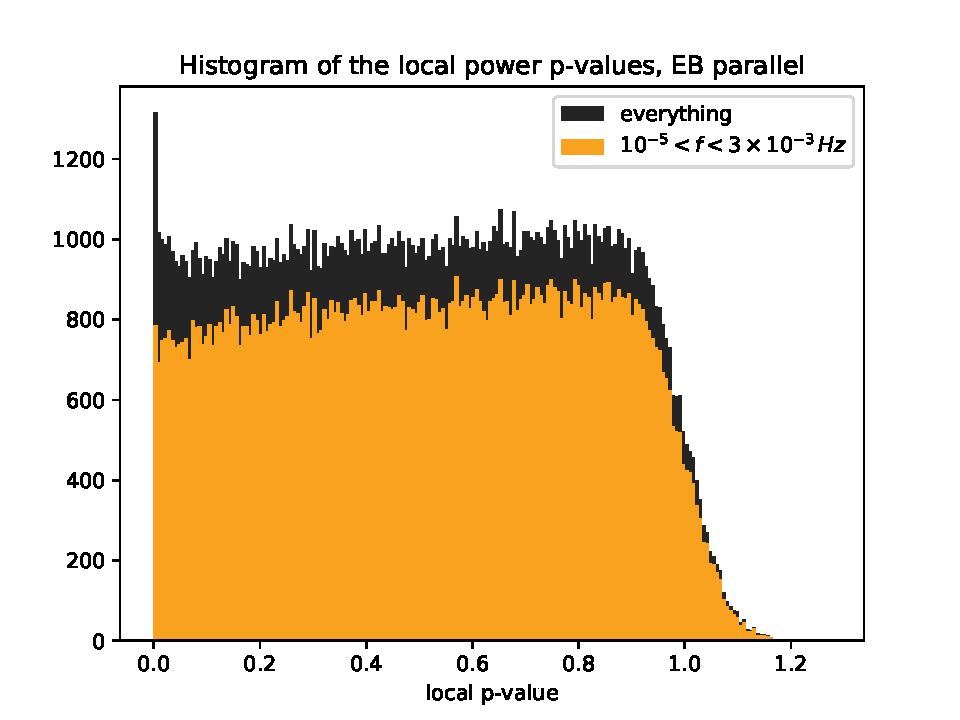
\includegraphics[width=0.9\linewidth]{gfx/axions/P_p-values.pdf}
  \caption{Accounting for the look-elsewhere effect for the parallel dataset. It provides the minimal local p-value -- global p-value transition. The fit with the model \dots gives the number of frequencies. \note{Prepare this histogram in a way, that the curves for all the datasets are shown. Then may need to normalise it.}}
  \label{fig:axions_P_p-values}
\end{figure}

\begin{figure}
  \centering
  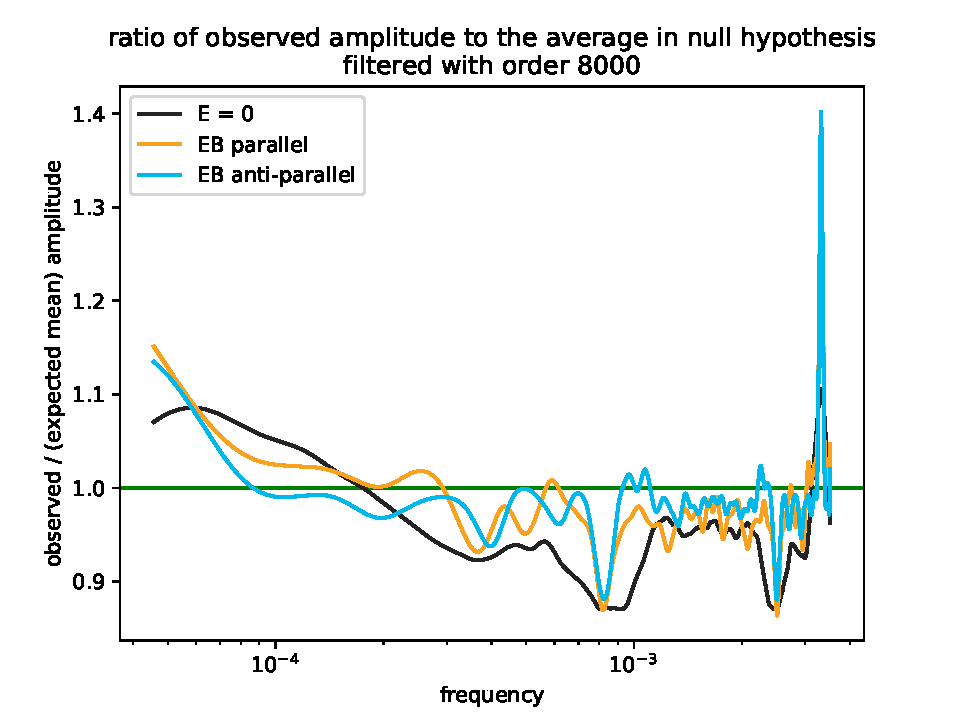
\includegraphics[width=0.9\linewidth]{gfx/axions/observed-predicted_power_ratio_filtered.pdf}
  \caption{Maybe mark the 1/300 seconds. Note, that because of the settling of the filter first $N$ points need to be dropped, so not whole range is plotted.}
  \label{fig:axions_observed-predicted_power_ratio_filtered}
\end{figure}



\section{Axion-Wind analysis}
The analysis described in this chapter so far concerned the scalar coupling of the axions to gluons, which looks like an oscillation in the electric dipole moment of the neutron.
Now we describe how we used the same data set and the same analysis techniques to look for a different coupling --- a vector one of axions to nucleons.

\begin{figure}
  \centering
  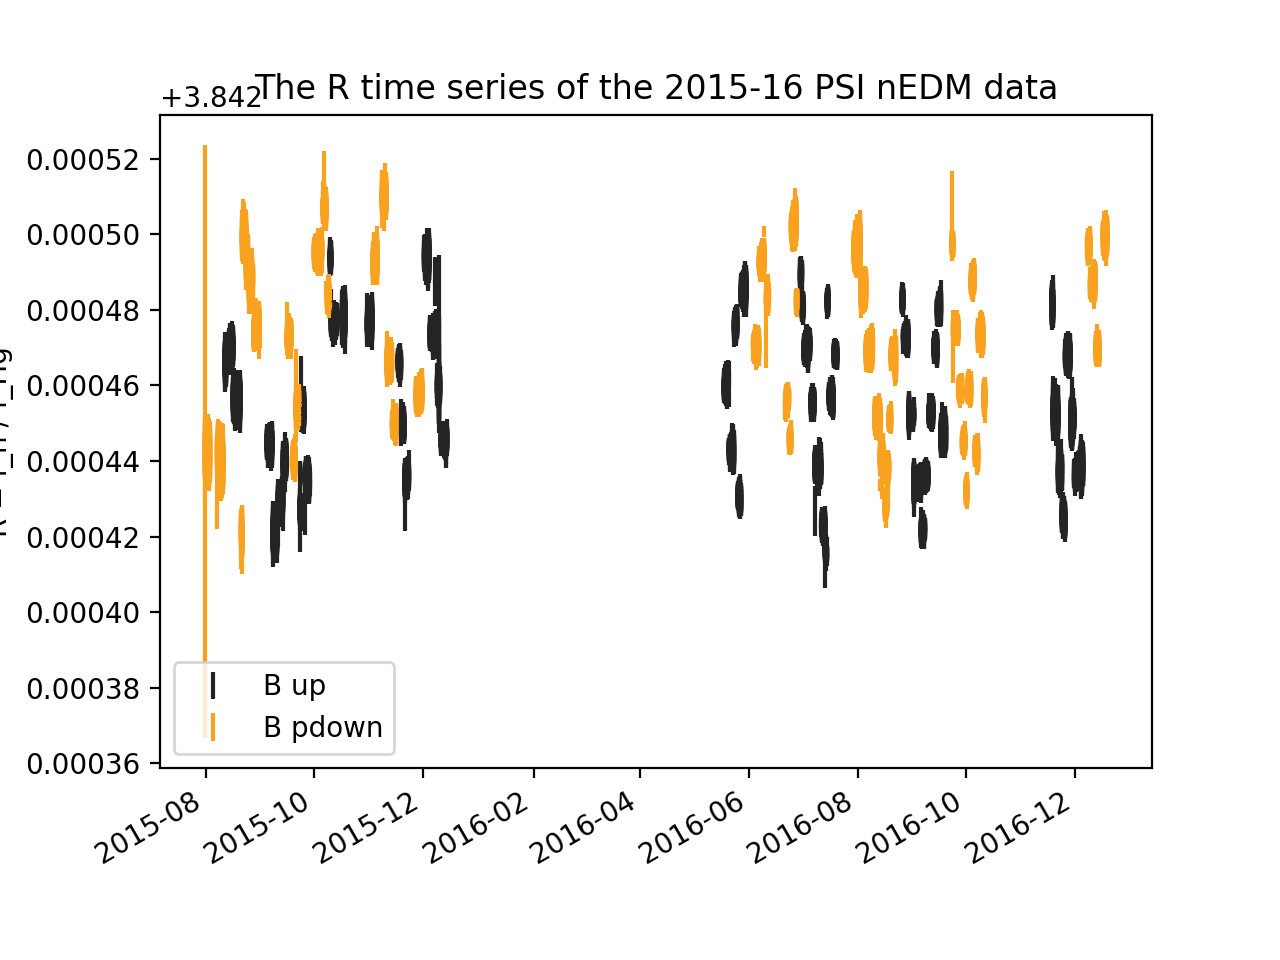
\includegraphics[width=0.9\linewidth]{gfx/axions/winddeltah4mm_time_domain.png}
  \caption{\ldots}
  \label{fig:axions_wind_time_domain}
\end{figure}

This coupling acts like an additional dynamic magnetic field. In this analysis the data are split based on the direction of the holding magnetic field $B_0$, as indicated in Fig.\,\ref{fig:axions_wind_time_domain}. The axion-wind coupling is insensitive to the electric field in the experiment.

The axion-wind coupling \note{ref to equation} is proportional to the projection of experiment's quantisation axis on the momentum of the axions.
Because the latter is due to the Earth traversing the galactic axion field in the Solar System's movement around the Milky Way's centre, the effect is called Axion-Wind. \note{Maybe a ref}
The Earth additionally spins, causing the effect to be modulated with the sidereal frequency $\Omega_\mathrm{sid}$.\footnote{Sidereal frequency is one of the Earth's spinning as seen in the reference of fixed stars.}
The modulation makes a signal in periodogram a triplet, with the central, highest, peak at the frequency of the oscillation of the axion field, and two additional ones, on either side, $\Omega_\mathrm{sid}$ away from the main peak.

Besides splitting the data on the direction of the magnetic field, rather than the relative direction of the magnetic and electric ones, the analysis is performed exactly in the same way as in the case of the search for the scalar axion-gluon coupling. The periodograms for the two datasets are presented in Fig.\,\ref{fig:axions_wind_Bup_detection} (magnetic field pointing upwards, relative to gravity) and Fig.\,\ref{fig:axions_wind_Bdown_detection} (pointing downwards).

\begin{figure}
  \centering
  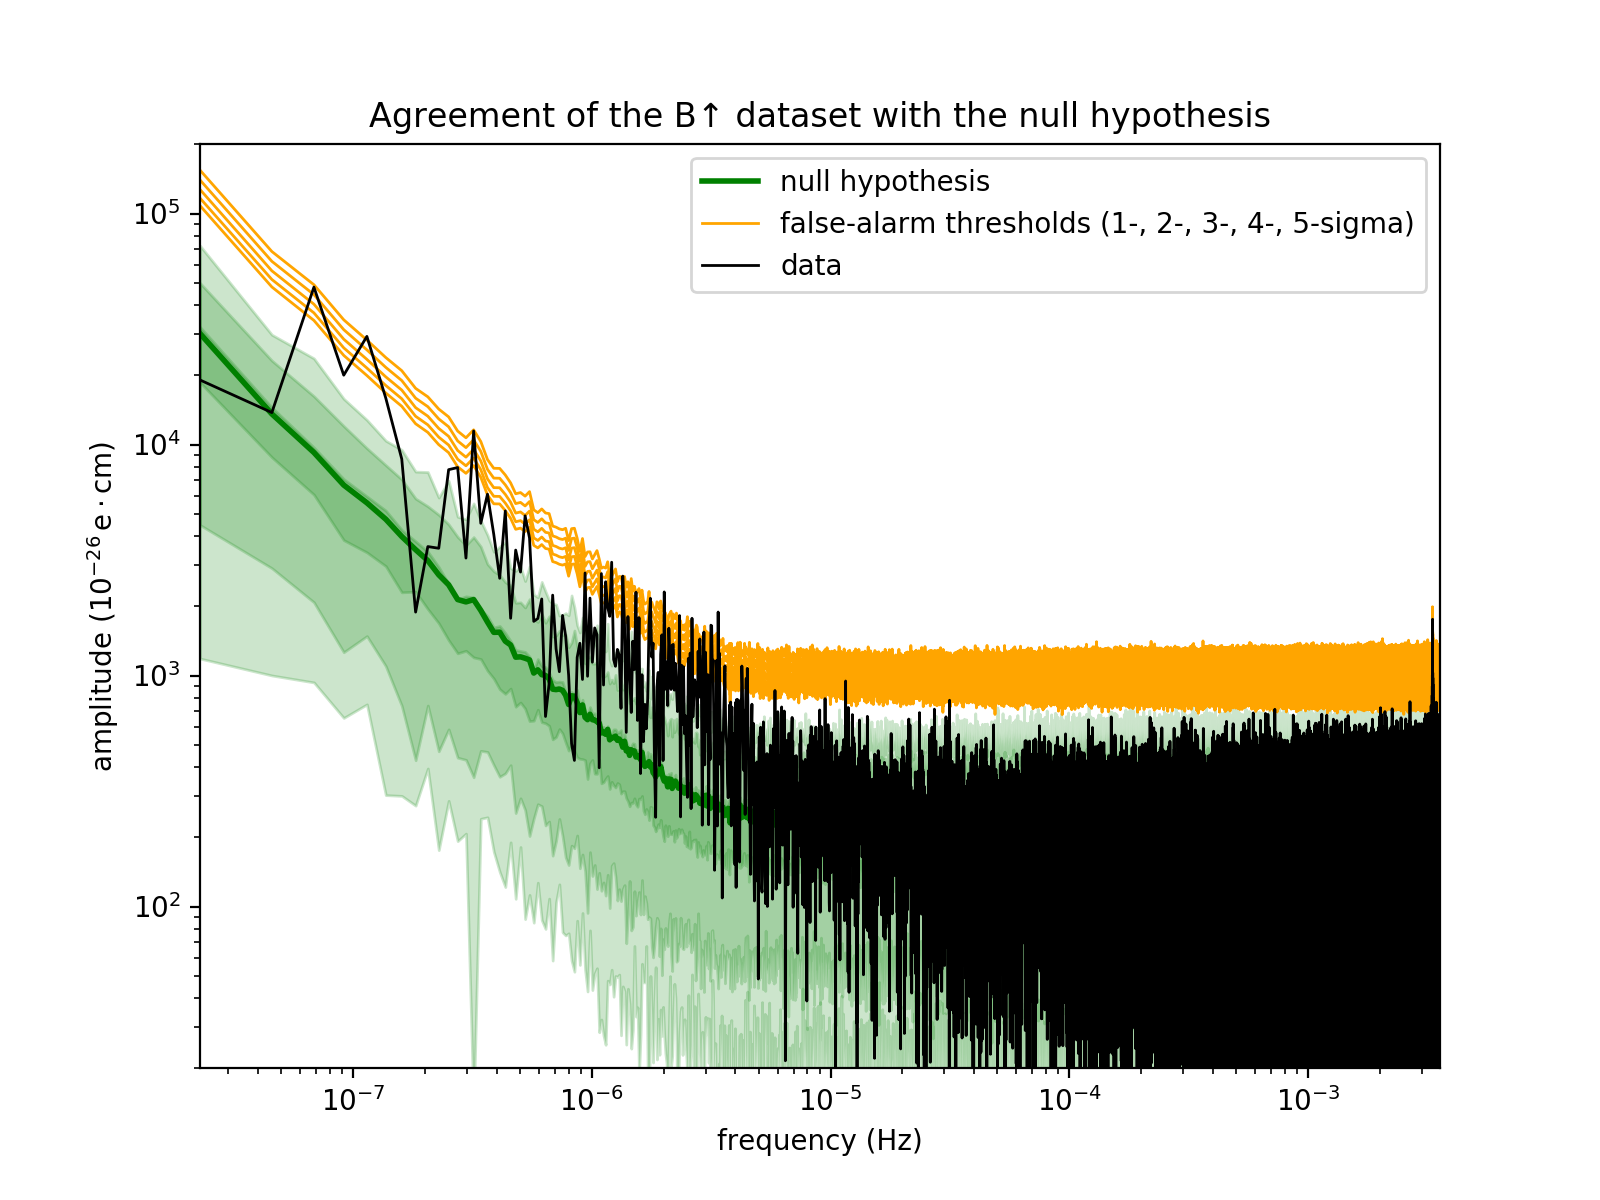
\includegraphics[width=0.9\linewidth]{gfx/axions/winddeltah4mm_Bup_detection.png}
  \caption{Maybe mark the 1/300 seconds. Note, that because of the settling of the filter first $N$ points need to be dropped, so not whole range is plotted.}
  \label{fig:axions_wind_Bup_detection}
\end{figure}

\begin{figure}
  \centering
  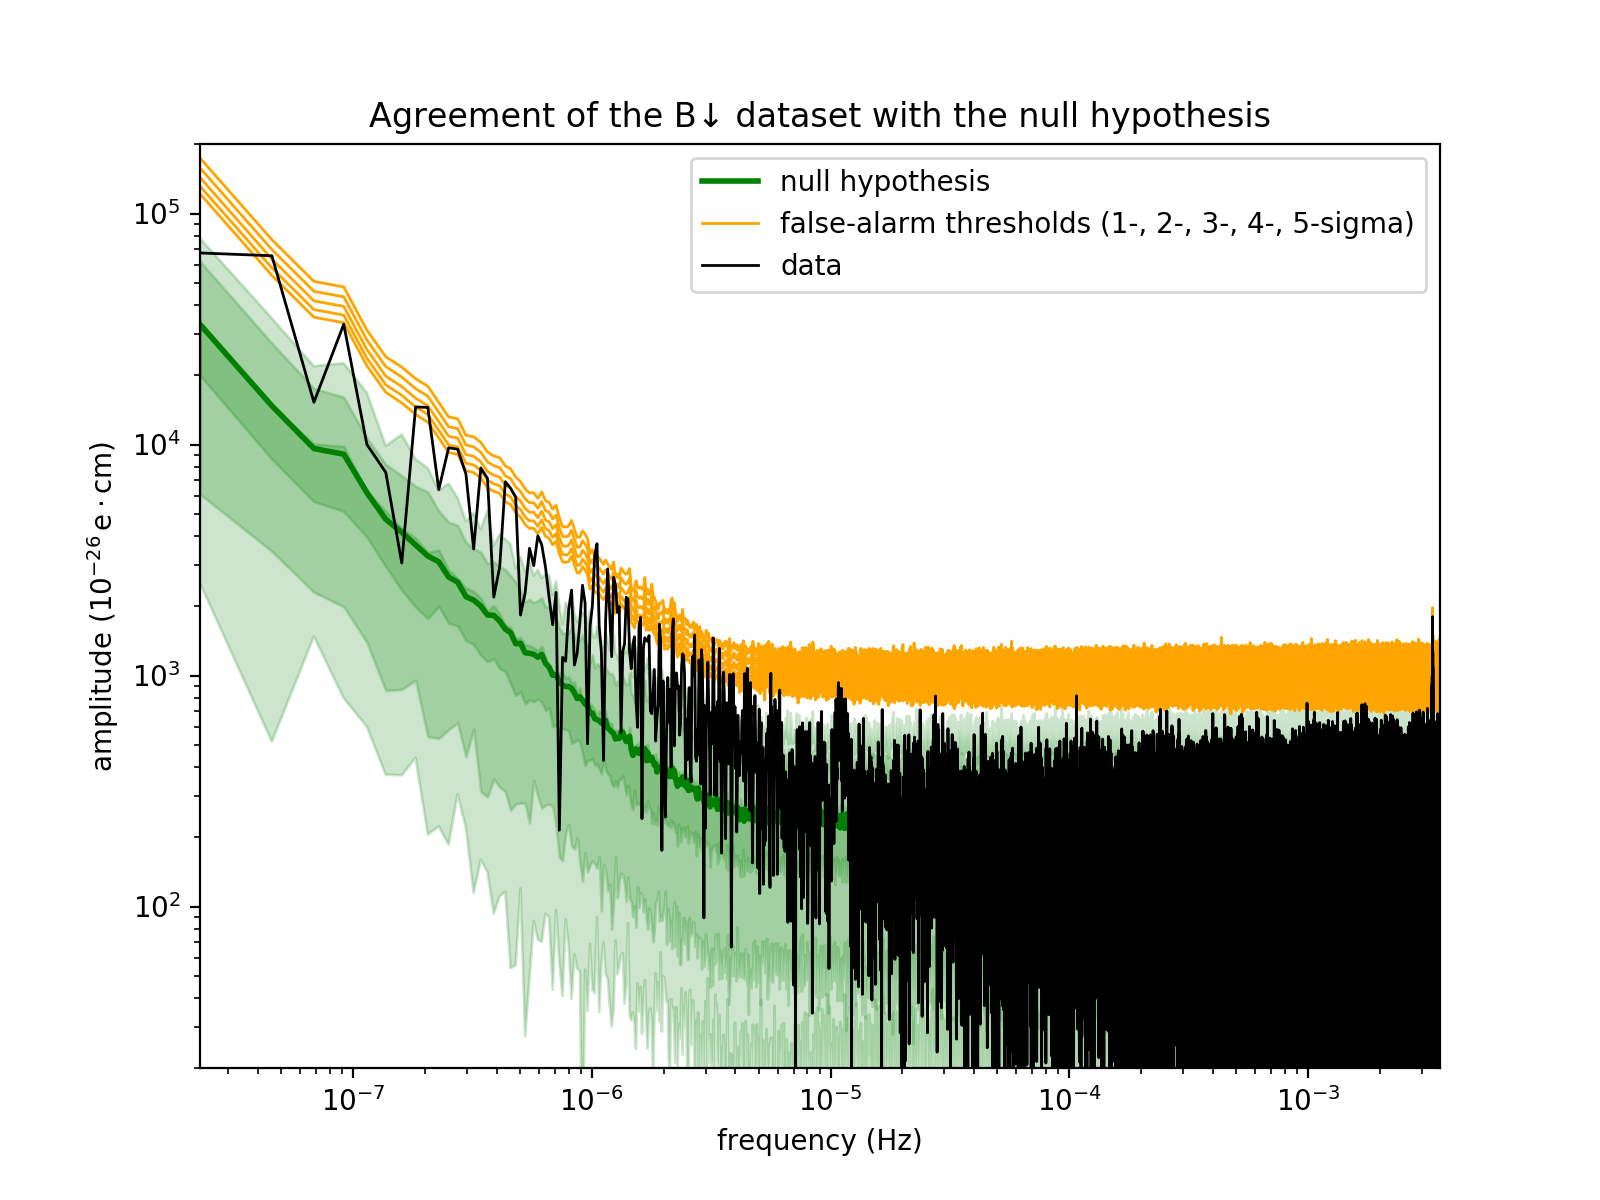
\includegraphics[width=0.9\linewidth]{gfx/axions/winddeltah4mm_Bdown_detection.png}
  \caption{\ldots}
  \label{fig:axions_wind_Bdown_detection}
\end{figure}

We see a lot of excesses (figures, already gradient-drift corrected), but none passes the detection criteria (the phase requirements in particular).

The lack of statistically significant signal compatible with the axion model allowed us to put limits on the axion-nucleon coupling, depicted in Fig.\,\ref{fig:axions_wind_limits}. \note{comment a bit on the other limits in the plot}

\begin{figure}
  \centering
  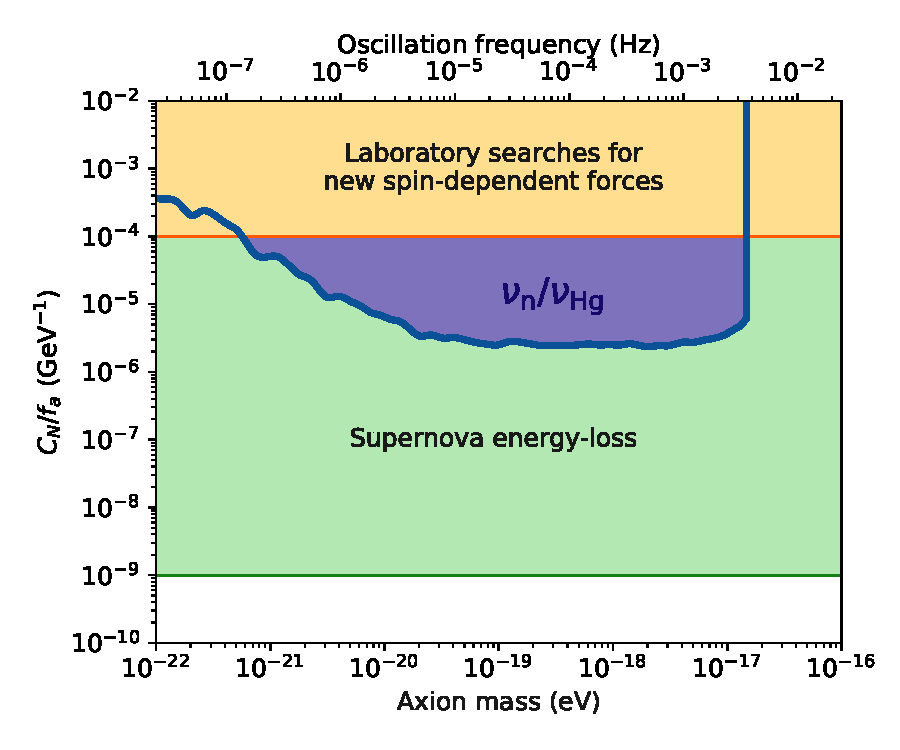
\includegraphics[width=0.9\linewidth]{gfx/axions/psi_ill_axion_wind_limits_v1.pdf}
  \caption{\ldots}
  \label{fig:axions_wind_limits}
\end{figure}



\section{Outlook}
There are three direction in which the nEDM-based axion dark matter search could continue.
To improve sensitivity vertically (be sensitive to more weekly coupled or less abundant axions) the overall sensitivty of the nEDM measurement would need to be improved.
Following the Eq\,\note{ref to the nEDM sensitivity formula}: more neutrons or higher electric field.
\marginpar{In Eq. $\alpha$ is already \ldots, precession time $T$ can only be improved so long --- it is fundamentally limited by the neutron life-time (give the number.)}
The global community already spares no effort to achieve that.
The second way is to improve sensitivity for slower oscillations, or lighter axions, limited by the span of the data set. For this analysis this are the four years of the ILL measurement. Combining the ILL and PSI data into one time series would improve it to \note{number}. It was not done at the time, because the PSI data were still blinded and the run-level analysis was still ongoing.
The third direction is the high-frequency, heavy-axions one. It is limited by the sampling frequency fo the system, the cycle repetition rate. The measurements could be conducted with a shorter cycle time (worsening the sensitivity, as the loss in Eq.\,\note{ref the nEDM sensitivity} is linear, and the gain from the statistics is a square root).
\marginpar{In PSI the cycles are synchronised to the pulses of the kicker magnet, redirecting the proton beam onto the target of the UCN source.}
However, it is hard to imagine going beyond ten-second range. A real improvement in this direction would require changing the principle of the measurement.




\section{Resonant oscillating nEDM search}
Many of the axion searches are resonant based. \note{some references}.
The standard instrument to look for an axion-photon coupling, called a haloscope \note{verity}, consists of ultra-low-noise resonant cavity, where axions can produce photons, detected with an antenna \note{is it an antenna?}.
At any given time the measurement is sensitive only to a narrow band of photon energies (or frequencies), the width given by the finesse \note{verity} of the cavity. To cover a wide range the tuning of the cavity is scanned. In this section an idea of a resonant oscillating nEDM search is pursued.

For polarised neturons in a magnetic field, a transverse oscillating coupling induces a coherent Rabi oscillation between the spin-up and spin-down states.
For example, a Ramsey cycle begins with a $\uppi$/2 flip, induced by an oscillating transverse magnetic field, its frequency tuned to the Larmor one and its length tuned such, that the Rabi oscillation stops when the polarisation is in the transverse plane. Should the nEDM oscillate, an oscillating transverse coupling can be achieved with a static magnetic field \emph{perpendicular} to the holding magnetic field. Then, if the frequency of the nEDM oscillation is tuned to the Larmor one, the neutrons would undergo a Rabi nutation, which could be detected.



First - just scanning.

Broad band possibility? It is like an adiabatic spin-flip, but without the oscillating field. The fact that the spin flip occurs, would indicate a presence of the field.